%
% related-work.tex
%
% Copyright (C) 2023 by Universidade Federal de Santa Catarina.
%
% Towards the Conception of GNSS Networks Based on Small Satellites
%
% This work is licensed under the Creative Commons Attribution-ShareAlike 4.0
% International License. To view a copy of this license,
% visit http://creativecommons.org/licenses/by-sa/4.0/.
%

%
% \brief Related works section.
%
% \author Gabriel Mariano Marcelino <gabriel.mm8@gmail.com>
%
% \version 1.1.0
%
% \date 2021/06/14
%

\chapter{Related Work} \label{ch:related-work}

%Este capítulo apresenta um resumo dos principais trabalhos relacionados e a situação atual das redes de GNSS no mundo, apresentando-se o histórico e status das redes atualmente em operação, e projetos atualmente em andamento e que possivelmente serão implementados ou entraram em operação no futuro, tanto com a utilização de satélites convencionais quanto com satélites de pequeno porte. Além de trabalhos relacionados estudando a viabilidade e possíveis soluções para a implantação destas redes através de uso de pequenos satélites e/ou mega-constelações.

This chapter presents a summary of the main related works and the current situation of GNSS networks in the world, presenting the history and status of the networks currently in operation, as well as ongoing projects that may be implemented or put into operation in the future, both using conventional satellites and small satellites. In addition, it includes related works studying the feasibility and possible solutions for the deployment of these networks through the use of small satellites and/or mega-constellations.

\section{Current GNSS networks}

%Atualmente existem quatro redes de GNSS em operação: GPS\nomenclature{\textbf{GPS}}{Global Positioning System}, GLONASS\nomenclature{\textbf{GLONASS}}{\textit{Globalnaya navigatsionnaya sputnikovaya sistema}}, Galileo e BDS\nomenclature{\textbf{BDS}}{BeiDou Navigation Satellite System}. Além de mais duas redes locais, que operam de forma limitada a uma região específica: QZSS\nomenclature{\textbf{QZSS}}{Quasi-Zenith Satellite System} e IRNSS\nomenclature{\textbf{IRNSS}}{Indian Regional Navigation Satellite System}. Abaixo, encontra-se uma descrição e mais informações sobre cada uma dessas redes.

Currently, there are four GNSS networks in operation: GPS\nomenclature{\textbf{GPS}}{Global Positioning System.}, GLONASS\nomenclature{\textbf{GLONASS}}{\textit{Globalnaya navigatsionnaya sputnikovaya sistema.}}, Galileo, and BDS\nomenclature{\textbf{BDS}}{BeiDou Navigation Satellite System.}. In addition to two local networks, which operate in a limited way to a specific region: QZSS\nomenclature{\textbf{QZSS}}{Quasi-Zenith Satellite System.} and IRNSS\nomenclature{\textbf{IRNSS}}{Indian Regional Navigation Satellite System.}. Below there is a description and further information about each of these networks.

\subsection{GPS}

%O GPS \cite{gps}, ou Global Positioning System, é o sistema de GNSS desenvolvido e mantido pelos Estados Unidos. Foi o primeiro sistema de navegação global por satélite a ser desenvolvido e entrar em operação, tendo o projeto sido iniciado no início da década de 1970, com os primeiros satélites lançados em 1978. A rede se tornou operacional em 1995 e teve custo total de 10 bilhões de dólares. Atualmente possuí 24 satélites em operação, operando a uma altitude de aproximadamente 20200 quilômetros (MEO\nomenclature{\textbf{MEO}}{Medium Earth Orbit}) e com a premissa de se ter sempre pelo menos quatro satélites cobrindo qualquer ponto do planeta \cite{el-rabbany2002}.

GPS \cite{gps}, or Global Positioning System, is the GNSS system developed and maintained by the United States. It was the first global satellite navigation system to be developed and put into operation, with the project starting in the early 1970s and the first satellites launched in 1978. The network became operational in 1995 and had a total cost of approximately 10 billion dollars. Currently, it has 24 satellites in operation, operating at an altitude of approximately 20,200 kilometers (MEO\nomenclature{\textbf{MEO}}{Medium Earth Orbit.}) and with the premise of always having at least four satellites covering any point on the planet. The 24 satellites are divided in six orbital planes, with four satellites per plane \cite{el-rabbany2002}.

%Atualmente o sistema é de uso civil e militar, mas até a década de 2000, o sistema possuía precisão propositalmente limitada para dispositivos de uso civil, sendo seu uso em capacidade máxima destinado somente a aplicações militares. Por questões de segurança, erros propositais eram induzidos aos sinais transmitidos de forma que receptores de uso geral não possuíssem precisão menor que 90 metros.

Currently, the system is used for both civilian and military purposes, but until the 2000s, the system deliberately had limited precision for civilian use devices, with its maximum capacity use intended only for military applications. For security reasons, intentional errors were induced into the transmitted signals so that general-use receivers did not have accuracy less than 90 meters.

%O GPS opera em três frequências diferentes: 1575,42, 1227,6 e 1176,45 MHz, com larguras de banda igual a 15,345, 11 e 12,5 MHz, respectivamente. Utilizando essas frequências, operam quatro tipos de sinais: L1 C/A, L1C, L2 C, L2 P e L5 (os sinais L2 C e L2 P operam na mesma frequência: 1227,6 MHz). Os sinais são transmitidos através da modulação BPSK.

GPS operates at three different frequencies: 1575.42, 1227.6, and 1176.45 MHz, with bandwidths of 15.345, 11, and 12.5 MHz, respectively. Four types of signals are used: L1 C/A, L1C, L2 C, L2 P, and L5 (L2 C and L2 P signals operate at the same frequency: 1227.6 MHz). The signals are transmitted through BPSK modulation.

To control the operation of the network, the ground segment of the system is divided into three groups: master control station (MCS\nomenclature{\textbf{MCS}}{Master Control Station.}), monitor stations and ground control stations. The MCS is composed of a single station lacated in Colorado Springs (Colorado, USA), and is the center of the GPS operations.

The monitor stations are composed by five stations with a precisely known locations, located in Colorado Spring (same place as the MCS), Hawaii, Kwajalein, Diego Garcia and Ascension Island. These monitor stations have a high-quality GPS receivers and high-precision cesium clocks, mainly for tracking all satellites of the network in real-time. Some of them are also equiped with uplinks for uploading telecommands and informations for the satellites, and all of them are operated remotely by the MCS.

The locations and stations of the ground segment of the GPS network is illustrated in \autoref{fig:gps-ground-segment}.

\begin{figure}[!ht]
    \begin{center}
        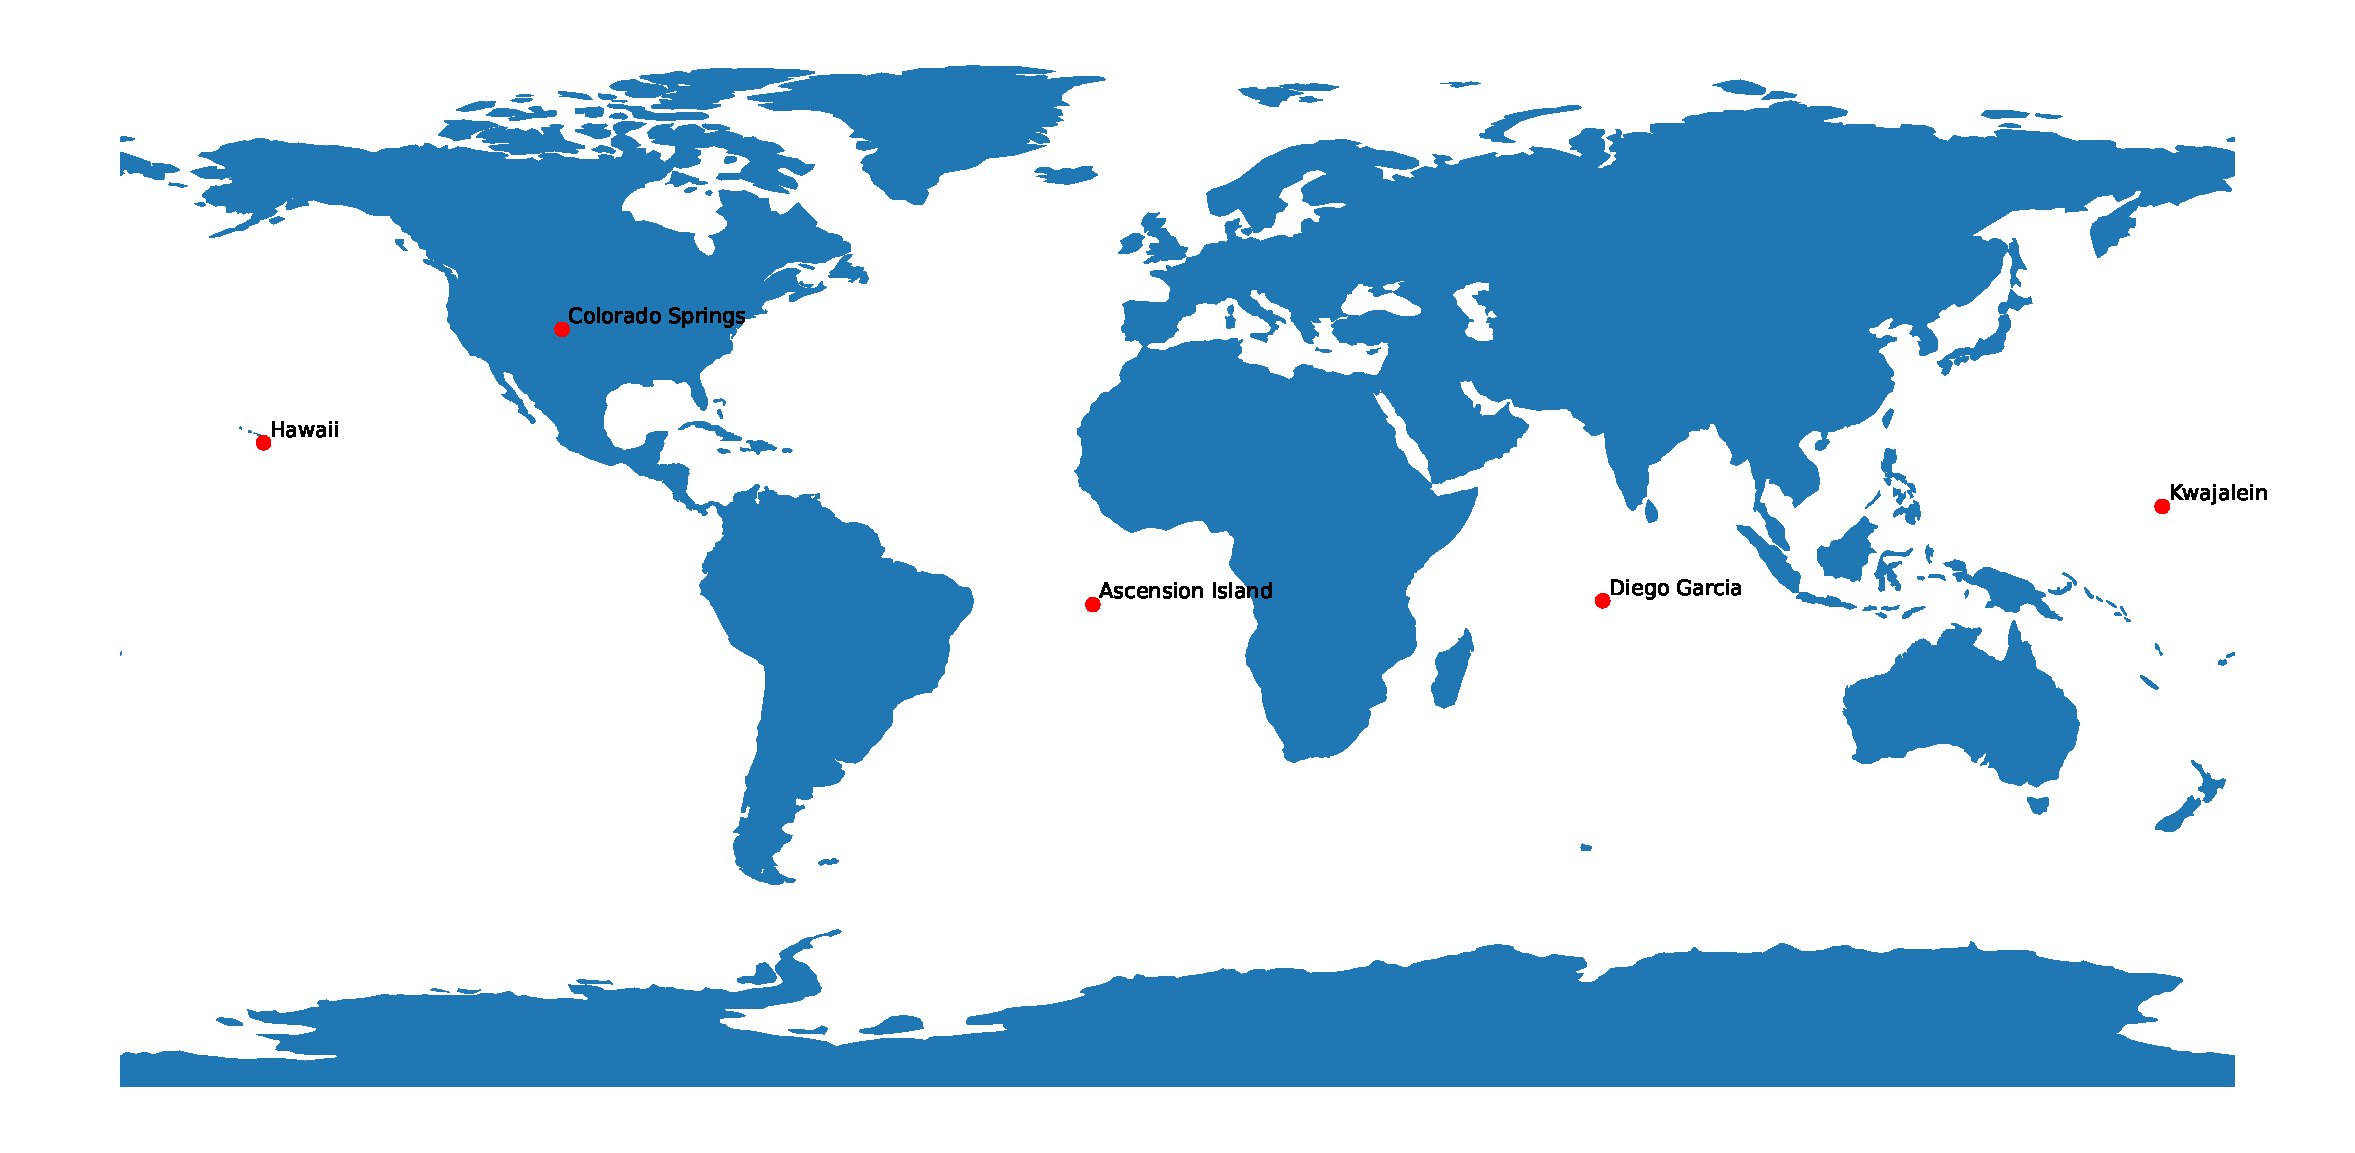
\includegraphics[width=\columnwidth]{curves/gps-ground-segment}
        \caption{Ground segment of the GPS network (adapted from \cite{el-rabbany2002}).}
        \label{fig:gps-ground-segment}
    \end{center}
\end{figure}

\subsection{GLONASS}

%O GLONASS, sigla de \textit{Globalnaya navigatsionnaya sputnikovaya sistema} (ou Sistema de Navegação Global por Satélite) \cite{glonass}, é o sistema de GNSS criado e mantido pela Rússia. Este foi o segundo sistema de navegação global a entrar em operação, logo após o GPS, ainda durante o período da União Soviética.

%O projeto começou a ser desenvolvido em 1976, ainda na União Soviética. A implantação do sistema iniciou em 1982, e foi até 1995. Este é o projeto é o mais caro mantido pela agência espacial russa (Roscosmos), consumindo atualmente um terço do seu orçamento.

%O GLONASS opera em uma órbita circula a uma altitude de 19100 km e com uma inclinação de 64,8$^{\circ}$, resultando em período de 11 horas e 15 minutos. Sendo um sistema desenvolvido principalmente para cobrir o território russo (mas além disso, com cobertura global), este é adequado para operações em altas latitudes, onde o GPS pode apresentar problemas \cite{polischuk2002}.

%O GLONASS opera com quatro tipos de sinais: L1 C/A (1598,0625-1609,3125 MHz), L2 C (1242,9375-1251,6875 MHz), L2 P (1242,9375-1251,6875 MHz) e L3 OC (1202,025 MHz). Da mesma forma que o GPS, os sinais são transmitidos através da modulação BPSK.

%Atualmente, é comum o uso de receptores que são compatíveis tanto com GPS quanto com o GLONASS. Desta forma, tem-se uma maior disponibilidade de satélites, fazendo com que tenha-se uma maior rapidez na obtenção dos dados de posicionamento e uma maior precisão destes dados. Receptores deste tipo são mais robustos que receptores operando em uma única rede \cite{angrisano2012}.

GLONASS, which stands for \textit{Globalnaya navigatsionnaya sputnikovaya sistema} (or Global Navigation Satellite System in english) \cite{glonass}, is the GNSS system created and maintained by Russia. This was the second global navigation system to enter operation, right after GPS, still during the Soviet Union period.

The project started to be developed in 1976, still in the Soviet Union, based on the experiences with the Doppler satellite system Tsikada \cite{hofmann-wellenhof2007}. The system deployment started in 1982 and went until 1995. This is the most expensive project maintained by the Russian space agency (Roscosmos), currently consuming one-third of its budget.

GLONASS is originally a military-use system, for this reason, few information about the system was made available to the public during its early days. In 1988, a paper with technical information about the system was presented. In 1995, the Russian government issued a decree making the system available for use worldwide, thus no longer being an exclusive system for the Russian armed forces \cite{hofmann-wellenhof2007}.

GLONASS operates in a circular orbit at an altitude of 19,100 km and with an inclination of 64.8$^\circ$, resulting in a period of 11 hours and 15 minutes. The constellation consists of 24 satellites in three orbital planes, with 21 satellites considered as active, and three as spare satellites. Each orbital plane has eight equally spaced satellites \cite{hofmann-wellenhof2007}. Being a system developed mainly to cover the Russian territory (but also with global coverage), it is suitable for operations at high latitudes, where GPS can present problems \cite{polischuk2002}.

GLONASS operates with four types of signals: L1 C/A (1598.0625-1609.3125 MHz), L2 C (1242.9375-1251.6875 MHz), L2 P (1242.9375-1251.6875 MHz), and L3 OC (1202.025 MHz). Similarly to GPS, the signals are transmitted through BPSK modulation.

The satellites of this system follows an specification list described as below \cite{hofmann-wellenhof2007}:

\begin{itemize}
    \item Lifetime of at least three years
    \item Satellites mass of 1,415 kg
    \item Mass of the payload of 180 kg
    \item Power supply of 1,000 W
    \item Power consumption of the payload of 600 W
    \item Clock precision of 5 $\times$ 10$^{-13}$
    \item Attitude control system with an accuracy of 0.5$^{\circ}$
    \item Pointing accuracy of the solar panel of 5$^{\circ}$
\end{itemize}

The ground segment of the system is mostly installed over Russian territory, but some stations are located in countries that were part of the Soviet Union. The system control center, where the entire system is coordinated, is located in a military complex at the Krasnoznamensk Space Center near Moscow. The system time is controlled by the central synchronizer, also located in the Moscow region. The telemetry and telecommand stations, where communication with the satellites of the constellation occurs, are composed of four stations installed over Russian territory: St. Petersburg, Schelkovo, Yenisseysk (Siberia), and Komsomolsk-na-Amure (Far East). There are also five supplementary laser stations located mostly outside of Russian territory: one in Komsomolsk-na-Amure (inside Russia) and four others in Kazakhstan, Ukraine (two stations), and Uzbekistan \cite{hofmann-wellenhof2007}.

Currently, the use of receivers that are compatible with both GPS and GLONASS is common. In this way, there is a greater availability of satellites, resulting in faster data acquisition and greater precision of this data. Receivers of this type are more robust than those operating on a single network \cite{angrisano2012}.

\subsection{Galileo}

%O Galileo é o sistema de GNSS criado pela união europeia e mantido pela Agência Espacial Europeia (ESA), que começou a sua operação em 2016. O projeto começou a ser desenvolvido em 1999 e teve como principal objetivo desenvolver um sistema de posicionamento global de alta precisão independente dos sistemas GPS e GLONASS, levando em conta principalmente razões políticas e militares.

Galileo is the GNSS system created by the European Union and maintained by the European Space Agency (ESA), which started its operation in 2016. The project began to be developed in 1999 and had as its main objective to develop a high-precision global positioning system independent of the GPS and GLONASS systems, taking into account mainly political and military reasons.

%O sistema operara oferencendo dois tipos de serviço: um de precisão mais baixa aberto e gratuito, e outro de precisão mais alta de uso limitado e restrito. A constelação completa do sistema Galileo é composta por 24 satélites.

The system offers two types of service: one with lower precision, open and free, and another with higher precision, limited and restricted use. The complete constellation of the Galileo system consists of 30 satellites, considering 3 as spare. They are divided into three orbital planes (nearly circular orbits, MEO) with an inclination of 56$^{\circ}$. Considering the nominal opearion, a minimum of six satellites are guaranteed to be viewed at any place of the world \cite{hofmann-wellenhof2007}.

%O sistema funciona através de três tipos de sinais: E1 (1575,42 MHz), E5 (1191,795 MHz) e E6 (1278,75 MHz). O sinal E5 é subdividido em dois outros: E5a (1176,45 MHz) e E5b (1207,14 MHz).

The system operates through three types of signals: E1 (1575.42 MHz), E5 (1191.795 MHz), and E6 (1278.75 MHz). The E5 signal is subdivided into two others: E5a (1176.45 MHz) and E5b (1207.14 MHz). The configuration of the signals are presented in \autoref{tab:galileo-signals}.

\begin{table*}[!ht]
    \centering
    \begin{tabular}{lcc}
        \toprule[1.5pt]
        \textbf{Signal} & \textbf{Frequency} & \textbf{Modulation} \\
        \midrule
        E1  & 1575,42 MHz & CBOC \\
        E5a & 1176,45 MHz & AltBOC \\
        E5b & 1207,14 MHz & AltBOC \\
        E6  & 1278,75 MHz & BPSK \\
        \bottomrule[1.5pt]
    \end{tabular}
    \caption{Galileo signals configuration.}
    \label{tab:galileo-signals}
\end{table*}

%Atualmente, boa parte dos receptores GNSS comerciais e de uso civil têm suporte a rede Galileo. Por exemplo, grande parte dos smartphones modernos têm capacidade de trabalhar com múltiplas redes de GNSS, sendo a Galileo uma delas.

The satellites of the Galileo system carry two types of payloads: the main navigation payload and the SAR\nomenclature{\textbf{SAR}}{Search And Rescue.} payload. The first one is responsible for transmitting the Galileo signals, including all the needed equipment for that and the L-band antenna. The second payload receives emergency signals from equipments on Earth, redirecting them to ground stations through the L-Band link. The Galileo satellites have a size of approximately 2.7 $\times$ 1.2 $\times$ 1.1 m, and a weight of 730 kg. Besides a predicted lifetime of 12 years. A block diagram of the satellites of the Galileo constellation is available in \autoref{fig:galileo-satellite-bd}.

\begin{figure}[!ht]
    \begin{center}
        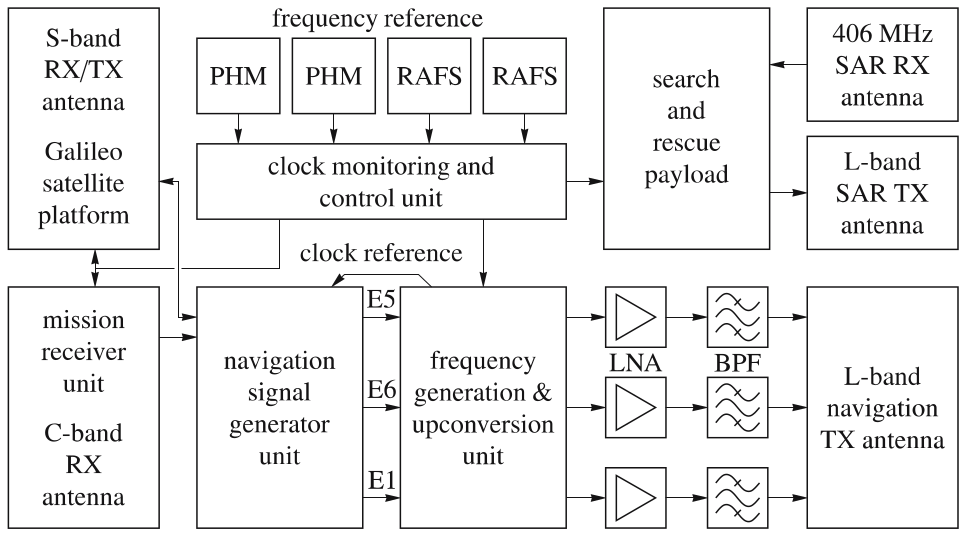
\includegraphics[width=\columnwidth]{figures/galileo-satellite-bd}
        \caption{Block diagram of a Galileo satellite \cite{hofmann-wellenhof2007}.}
        \label{fig:galileo-satellite-bd}
    \end{center}
\end{figure}

The ground segment is composed by:

\begin{itemize}
    \item Two control centers (Ground Control Center, or GCC)
    \item Five telemetry, tracking and control stations (TT\&C)
    \item Nine uplink stations operating in C-Band (ULS)
    \item Aproximately 40 sensor stations (GSS)
\end{itemize}

A map with the stations of the ground segment of the Galileo system is presented in \autoref{fig:galileo-ground-segment}.

\begin{figure}[!ht]
    \begin{center}
        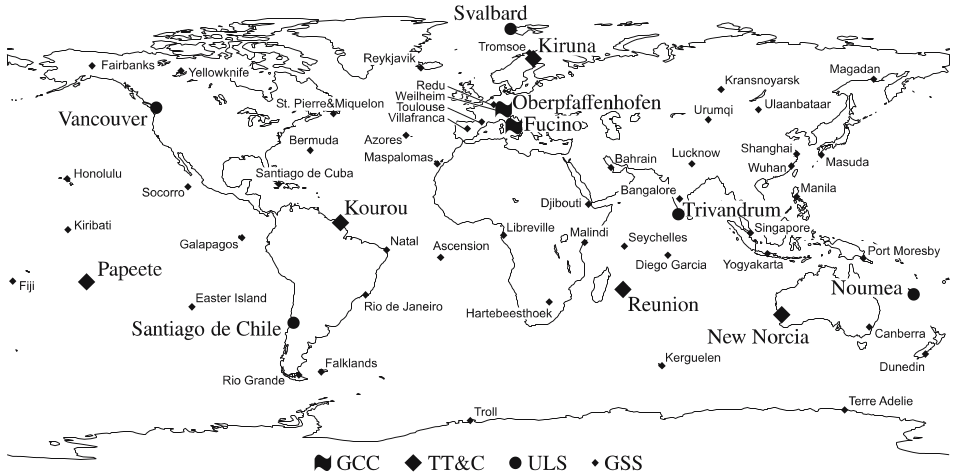
\includegraphics[width=\columnwidth]{figures/galileo-ground-segment}
        \caption{Ground segment of the Galileo system \cite{hofmann-wellenhof2007}.}
        \label{fig:galileo-ground-segment}
    \end{center}
\end{figure}

As can be seen, the ground infrastructure of the Galileo system highly robust in comparison with the other gelolocalization systems.

Currently, a large portion of commercial and civil GNSS receivers support the Galileo network. For example, most modern smartphones have the capability to work with multiple GNSS networks, including Galileo.

\subsection{BDS}

%O \textit{BeiDou Navigation Satellite System}, ou BDS \cite{beidou}, é o sistema de GNSS chinês.

%BeiDou, or BDS, is a global GNSS owned and operated by the People's Republic of China. BDS was formally commissioned in 2020. The operational system consists of 35 satellites. BDS was previously called Compass.

The Beidou Navigation Satellite System (BDS) \cite{beidou} a global navigation satellite system (GNSS) developed by China. Beidou, which means “Big Dipper” in Chinese, is also known as the Chinese Compass. The system consists of two separate satellite constellations: the regional Beidou-1 system and the global Beidou-2 system, which became fully operational in 2020.

The Beidou-1 system, which consists of four satellites, started operating in 2000. The Asia-Pacific area and China are its primary markets for positioning, navigation, and timing services. The GPS and GLONASS systems are compatible with the two frequencies used by the system, L1 and L2. A location accuracy of roughly 10 meters horizontally and 15 meters vertically, as well as a timing accuracy of roughly 10 nanoseconds, are provided by the Beidou-1 system.

There are 35 satellites total in the global Beidou-2 constellation, both geostationary and non-geostationary. The system offers positioning, navigation, and timing services with global coverage. Three frequencies—L1, L2, and L5—are used by the system for operation, and they are all compatible with other GNSS systems. The Beidou-2 system offers timing accuracy of around 20 to 30 nanoseconds, and positioning accuracy of roughly 2.5 meters horizontally and 5 meters vertically.

The Beidou system is made to be used for a variety of purposes, including commercial, civil, and military ones. In fields including transportation, surveying and mapping, precision agriculture, and disaster assistance, it is anticipated to have significant uses.

The Beidou Satellite-Based Augmentation System is a satellite-based augmentation system (SBAS\nomenclature{\textbf{SBAS}}{Satellite-Based Augmentation System.}) that the Beidou system offers in addition to GNSS capabilities (BDSBAS). The Beidou system's positioning, navigation, and timing services will be more accurate and dependable thanks to the BDSBAS.

Overall, China's development of cutting-edge space technologies has advanced thanks to the Beidou GNSS system. The technology is positioned to have a significant impact on navigation and location in the future thanks to its wide variety of applications and global coverage.

\section{Local networks}

Another type of network also in operation today is the network that operates locally, covering a specific region of the globe, called Regional Navigation Satellite System (RNSS\nomenclature{\textbf{RNSS}}{Regional Navigation Satellite System.}). With this characteristic, there are two in operation nowadays: QZSS and IRNSS networks. Both are described below.

\subsection{QZSS}

%The Quasi-Zenith Satellite System \cite{qzss} (QZSS, or also know as Michibiki) is a local positioning system developed by the Japanese government covering part of Asia and Oceania, focusing primordially on the japanese territory. The objective of this system is to improve the GPS system coverage in the region with higher stability and precision. Currently, the system is composed by four satellites (QZS-1, 2, 3 and 4) and it is compatible with the GPS, but an independent system is also planned to be operational with seven satellites in 2023.

%The QZSS operates with one geostationaty satellite and three in a Tundra highly inclined, slightly elliptical, geosynchronous orbit, with each satellite 120$^{\circ}$ apart from each other. quasi-zenith orbit (QZO\nomenclature{\textbf{QZO}}{Quasi-Zenith Orbit}) scheme. This orbit is illustrade in \autoref{fig:qzss-orbit}.

The Quasi-Zenith Satellite System (QZSS) \cite{qzss} is a satellite-based positioning system developed by the Japanese government. It consists of a constellation of four satellites, one in geostationary orbit and three in a highly inclined elliptical orbit that covers Japan and the surrounding regions.

The QZSS system is designed to provide enhanced positioning accuracy and reliability, particularly in urban areas and mountainous terrain where satellite signals may be obstructed or weakened. The QZSS system is also designed to work in conjunction with other satellite positioning systems, such as GPS and GLONASS, to improve overall accuracy and reduce signal interference.

One of the unique features of the QZSS system is its use of a ``quasi-zenith'' orbit for its three inclined satellites. This means that the satellites spend a significant amount of time near the zenith, or highest point in the sky, which allows them to broadcast signals that are less obstructed by buildings and other obstructions. This orbit is illustrade in \autoref{fig:qzss-orbit}.

\begin{figure}[!ht]
    \begin{center}
        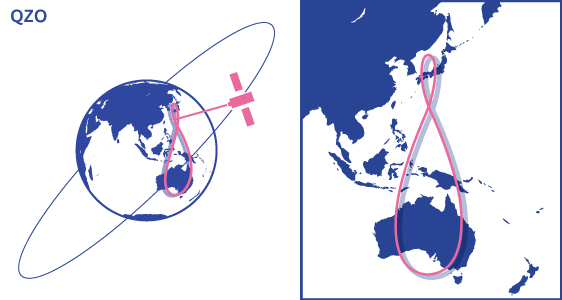
\includegraphics[width=0.8\columnwidth]{figures/qzss-orbit}
        \caption{Quasi-Zenith orbit of the QZSS network \cite{qzss}.}
        \label{fig:qzss-orbit}
    \end{center}
\end{figure}

The orbital elements of the QZSS satellites are available in \autoref{tab:qzss-orbit-config}.

\begin{table*}[!ht]
    \centering
    \begin{tabular}{lc}
        \toprule[1.5pt]
        \textbf{Keplerian Elements} & \textbf{Value} \\
        \midrule
        Epoch                                   & 26 December 2009, 12:00 UTC \\
        Semimajor                               & 42164 km \\
        Eccentricity                            & $0,075 \pm 0,015$ \\
        Inclination                             & $43 \pm 4^{\circ}$ \\
        Right ascension of the ascending node   & $195^{\circ}$ \\
        Argument of perigee                     & $270 \pm 2^{\circ}$ \\
        Mean anomaly                            & $305^{\circ}$ \\
        Central longitude of ground trace       & $135\ E \pm 5^{\circ}$ \\
        \bottomrule[1.5pt]
    \end{tabular}
    \caption{Orbit configuration of the QZSS.}
    \label{tab:qzss-orbit-config}
\end{table*}

The QZSS system is used for a variety of applications, including transportation, disaster response, agriculture, and surveying. The system has also been integrated into some consumer devices, such as smartphones and car navigation systems.

The QZSS system is considered an important strategic asset for Japan, and the government has plans to expand the constellation to seven satellites by 2023. This expansion will further enhance the system's accuracy and reliability and make it an even more valuable resource for users in Japan and beyond.

\subsection{IRNSS}

%The IRNSS (Indian Regional Navigation Satellite System) \cite{irnss} is a regional and independent nagivation system developed and maintained by India, focusing on covering mainly its territory. This network is currently composed by a constellation of seven satellites, three in a geostationaty orbit, and four in a geosynchronous orbit.

%IRNSS is a regional GNSS owned and operated by the Government of India. IRNSS is an autonomous system designed to cover the Indian region and 1500 km around the Indian mainland. The system consists of 7 satellites. In 2016, India renamed IRNSS as the Navigation Indian Constellation (NavIC, meaning ``sailor'' or ``navigator'').

The Indian Regional Navigation Satellite System (IRNSS) \cite{irnss}, also known as NavIC (Navigation with Indian Constellation), is a satellite-based positioning system developed by the Indian Space Research Organisation (ISRO). NavIC is designed to provide accurate and reliable positioning services to users in India and the surrounding regions.

The system consists of a constellation of seven satellites in orbit, three in geostationary orbit and four in geosynchronous orbit, covering the entire Indian subcontinent and extending up to 1,500 kilometers beyond its borders. NavIC is capable of providing a position accuracy of up to 5 meters, and the system is compatible with both GPS and GLONASS, allowing for greater redundancy and improved accuracy. A diagram of the IRNSS with the coverage area and the satellites can be seen in \autoref{fig:irnss}.

\begin{figure}[!ht]
    \begin{center}
        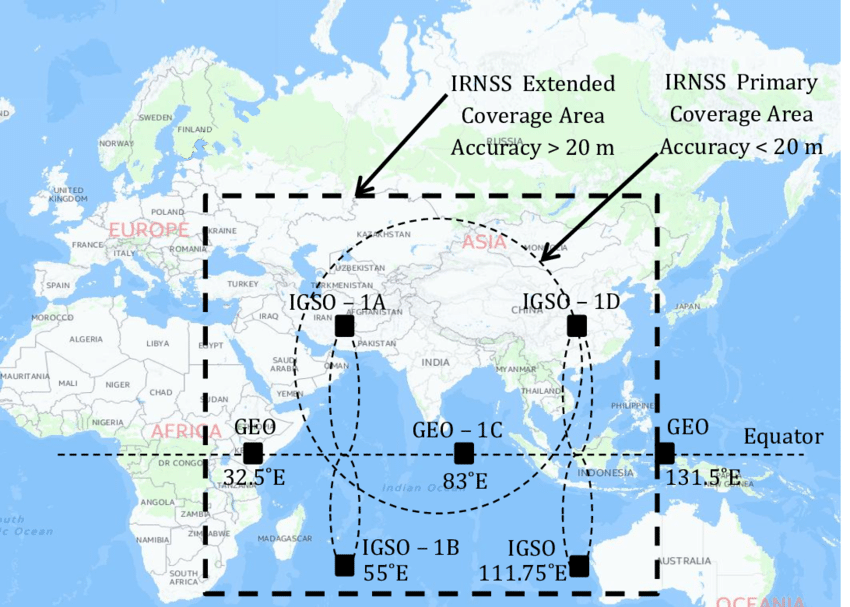
\includegraphics[width=0.8\columnwidth]{figures/irnss}
        \caption{IRNSS satellites and coverage of the system (adapted from \cite{thombre2015}).}
        \label{fig:irnss}
    \end{center}
\end{figure}

NavIC offers a wide range of applications, including vehicle tracking, maritime navigation, disaster management, and location-based services. The system is particularly useful in rural and remote areas of India, where traditional navigation systems may be unreliable or unavailable.

The Indian government has made NavIC available for civilian use, and several companies are already integrating the technology into their products and services. With the growing demand for accurate and reliable positioning information, NavIC is poised to become a major player in the global navigation satellite system market.

\subsection{KPS}

The Korea Positioning System (KPS\nomenclature{\textbf{KPS}}{Korea Positioning System.}) \cite{choi2020} is a satellite-based navigation system developed by the South Korean government. The KPS system is designed to provide positioning, navigation, and timing (PNT) services to users in South Korea and the surrounding regions.

%\begin{itemize}
%    \item GPS is a key component of the Korean national infrastructure, such as roads, power grid, timing, and national security
%    \item In the case of a looming crisis such as a conflict, signals can be blocked by countries with own GNSS system to prevent their enemy forces from using them
%    \item However, Korea does not have any navigation satellites, so totally depends on GNSS systems of other countries like GPS
%    \item This possibility necessitated the development of KPS
%\end{itemize}

%The Global Positioning System (GPS) is an essential technology for many countries, including South Korea. It plays a crucial role in the Korean national infrastructure, such as roads, power grids, timing, and national security.

One of the motivations for the development of this system, in that in times of crisis, such as a military conflict, countries with their own GNSS system could block the signals to prevent their enemy forces from using them. This situation raises concerns for South Korea, which relies entirely on GPS and other foreign GNSS systems. To address this issue, South Korea is developing its own GNSS system. The KPS aims to provide more accurate and reliable positioning information for Korean users, especially during emergencies when GPS signals could be blocked.

The KPS is also expected to promote technological independence and enhance the competitiveness of the Korean space industry. Moreover, it will contribute to the development of various industries that rely on positioning information, such as transportation, logistics, and agriculture.

In summary, the development of KPS is a significant step towards securing the nation's technological independence and strengthening its national security. With the launch of the KPS system, South Korea will join the group of countries with their own GNSS system. This system is still under development and is expected to be operational in the coming years.

\section{Comparison between systems}

Considering the information presented above about the navigation systems currently in operation (or already in implantation), \autoref{tab:networks-comparison} compares the main characteristics of all the systems presented.

\begin{landscape}

\begin{table*}[!ht]
    \centering
    \begin{tabular}{lccccccc}
        \toprule[1.5pt]
        \multirow{2}{*}{\textbf{Characteristic}} & \multicolumn{7}{c}{\textbf{Network}} \\
                                                 & \textbf{GPS} & \textbf{GLONASS} & \textbf{Galileo} & \textbf{BDS} & \textbf{QZSS} & \textbf{IRNSS} & \textbf{KPS} \\
        \midrule
        Coverage      & Global        & Global      & Global         & Global      & Regional    & Regional    & Regional \\
        Country       & United States & Russia      & European Union & China       & Japan       & India       & South Korea\\
        Satellites    & 32            & 24          & 30             & 30          & 4           & 7           & 3 \\
        Orbit         & MEO           & MEO         & MEO            & MEO         & GEO         & GEO/MEO     & LEO \\
        Altitude [km] & 20200         & 19100       & 23200          & 21000       & 39000       & 36000       & 1000 \\
        Bands         & L1, L2, L5    & L1, L2      & E1, E5a, E5b   & B1, B2, B3  & L1, L2C, L5 & L5, S       & K \\
        Launch year   & 1978          & 1982        & 2016           & 2000        & 2010        & 2013        & 2021 \\
        Accuracy [m]  & 5-10          & 5-10        & 1-5            & 5-10        & 1-5         & 5-10        & 5-10 \\
        Status        & Operational   & Operational & Operational    & Operational & Operational & Operational & Planned \\
        \bottomrule[1.5pt]
    \end{tabular}
    \caption{Comparison between the main global and regional navigation networks (situation in 2023).}
    \label{tab:networks-comparison}
\end{table*}

\end{landscape}

%        \multirow{6}{*}{Frequency [MHz]} & 1575,42 (L1 C/A)  & 1598,0625-1609,3125 (L1 C/A) & 1575,42 (E1)         & 1561,098 (B1l) & 1575,42 (L1 C/A/S) & 1176,45 (L5) \\
%                                         & 1227,6 (L2 C/P)   & 1242,9375-1251,6875 (L2 C/P) & 1176,45 (E5a)        & 1207,14 (B2l)  & 1227,6 (L2C)       &  \\
%                                         & 1176,45 (L5)      & 1202,025            (L3 OC)  & 1207,14 (E5b)        & 1268,52 (B3l)  & 1176,45 (L5)       &  \\
%                                         &                   &                              & 1191,795 (E5 AltBOC) & 1575,42 (B1C)  & 1278,75 (L6)       &  \\
%                                         &                   &                              & 1275,75 (E6)         & 1176,45 (B2a)  &                    &  \\
%                                         &                   &                              &                      & 1207,14 (B2b)  &                    &  \\

\section{Experimental GNSS networks}

%Recentemente, com o avanço dos nanossatélites, o crescimento de dispositivos com conectividade e a Internet das coisas (IoT), começou a surgir ideias de implantação de redes privadas e em baixa órbita de sistemas de GNSS, seja para atender propósitos específicos ou de uso geral. Considerando, começam a surgir iniciativas de empresas para a utilização de pequenos satélites para esse tipo de aplicação, o que vai de encontro a ideia principal deste trabalho.

Recently, with the advancement of nanosatellites, the growth of devices with connectivity and the Internet of Things (IoT), ideas for deploying private and low-orbit GNSS systems networks have emerged, either to serve specific or general purposes. Considering this, companies are starting to take initiatives to use small satellites for this type of application, which aligns with the main idea of this work.

%Dentre essas iniciativas, pode-se destacar duas startups que possuem propostas similares: TrustPoint\footnote{\href{https://www.trustpointgps.com/}{https://www.trustpointgps.com/}} e Xona Space Systems\footnote{\href{https://www.xonaspace.com/}{https://www.xonaspace.com/}}.

Among these initiatives, two startups with similar proposals can be highlighted: TrustPoint\footnote{\href{https://www.trustpointgps.com/}{https://www.trustpointgps.com/}} and Xona Space Systems\footnote{\href{https://www.xonaspace.com/}{https://www.xonaspace.com/}}.

%A primeira tem como proposta a criação de uma rede GNSS totalmente de uso comercial e com melhorias em relação ao GPS atual, como aumento de desempenho, melhorias de segurança e maior robustez. Mais especificamente, a proposta inclui um sistema anti-spoof and anti-jam, e um tempo menor para fixar o sinal. Além disso, para a implementação da rede propõe-se o uso de satélites de pequeno porte, do tipo microssatélite.

The first initiative proposes the creation of a completely commercial GNSS network with improvements over the current GPS, such as increased performance, improved security, and greater robustness. More specifically, the proposal includes an anti-spoof and anti-jam system, and a shorter time to fix the signal. In addition, the implementation of the network proposes the use of small satellites, such as microsatellites.

%Já a segunda \cite{aarestad2020}, propõe a implantação de redes privadas de GNSS, utilizando satélites em baixa órbita. Uma imagem conceitual de um dos satélites da rede pode ser vista na \autoref{fig:xona-satellite}.

The second one proposes the deployment of private GNSS networks, using satellites in low Earth orbit \cite{reid2020} \cite{reid2023}. A conceptual image of one of the network satellites can be seen in Figure \ref{fig:xona-satellite}.

\begin{figure}[!ht]
    \begin{center}
        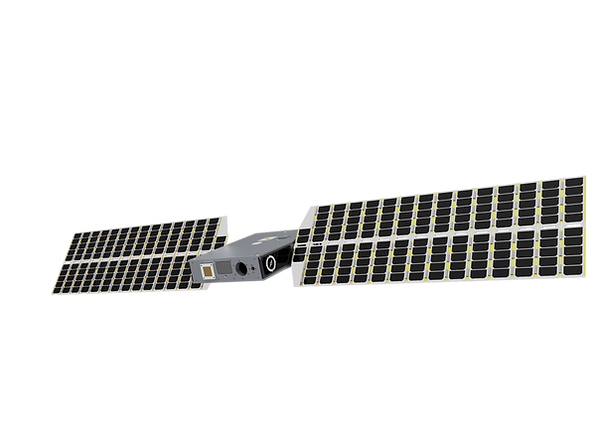
\includegraphics[width=0.8\columnwidth]{figures/xona-satellite}
        \caption{Xona Space Systems conceptual satellite.}
        \label{fig:xona-satellite}
    \end{center}
\end{figure}

%Considerando-se que ainda são projetos em estágio inicial e sendo desenvolvidos por empresas, não encontra-se disponível de forma pública informações mais técnicas e detalhadas sobre essas duas redes.

%Outros trabalhos ainda em fase pesquisa, também discutem a fusão de serviços de GNSS com outros tipos de serviço de telecomunicação, como por exemplo a adição de uma rede GNSS em megaconstelações como por exemplo a Starlink \cite{iannucci2022}.

Considering that they are still early-stage projects being developed by companies, more technical and detailed information about these two networks is not publicly available.

\section{Related works}

%Além das redes já consolidadas operando em órbitas mais altas e baseadas em satélites de grandes porte, há alguns trabalhos focados em tópicos específicos sobre a implantação de redes de geolocalização.

In addition to the already established networks operating in higher orbits and based on large satellites, there are some studies focused on specific topics regarding the deployment of geolocation networks.

Other research works still in progress also discuss the fusion of GNSS services with other types of telecommunication services, such as the addition of a GNSS network in mega-constellations like Starlink \cite{iannucci2022}.

%Já o trabalho de \cite{reid2018} apresenta um estudo sobre como constelações de satélites operando em órbita baixa (LEO) podem ser utilizadas para sistemas de navegação. O trabalho destaca as vantagens desse tipo de sistema, como por exemplo a operação com sinais com maior potência, o que permite uma melhor recepção em ambientes fechados, e uma maior robustez contra jamming. O trabalho também cita a principal desvantagem de sistemas operando nessas órbitas: a necessidade de um número maior de satélites para se obter uma cobertura global. Outro aspecto discutido é a menor incidência de radiação ionizante em órbitas baixas, o que torna possível por exemplo a utilização de componentes COTS\nomenclature{\textbf{COTS}}{Commercial-Off-The-Shelf.} (Commercial-Off-The-Shelf).

%Também existem trabalhos que exploram a utilização das redes de GNSS atuais em outros corpos estelares, como por exemplo a Lua \cite{capuano2015} \cite{delepaut2020}.

The work of \cite{reid2018} presents a study on how constellations of satellites operating in low Earth orbit (LEO) can be used for navigation systems. The paper highlights the advantages of this type of system, such as operating with higher power signals, which allows for better reception in indoor environments, and greater robustness against jamming. The work also mentions the main disadvantage of systems operating in these orbits: the need for a larger number of satellites to achieve global coverage. Another aspect discussed is the lower incidence of ionizing radiation in low orbits, which makes it possible, for example, to use Commercial-Off-The-Shelf (COTS\nomenclature{\textbf{COTS}}{Commercial-Off-The-Shelf.}) components.

There are also studies that explore the use of current GNSS networks on other celestial bodies, such as the Moon \cite{capuano2015} \cite{delepaut2020}.

\subsection{LoRa modulation}

%Um tipo de modulação com o uso em crescimento nos últimos anos, principalmente em aplicações envolvendo IoT, é a LoRa. Recentemente, além do uso em aplicações terrestres, também vem se difundindo o uso dessa modulação em satélites, especialmente CubeSats operando em órbita baixa. Um dos usos que pode se destacar é na coleta de dados de plataformas instaladas em solo \cite{anantachaisilp2020}.

%Além das características que a tornam ideal para comunicações de longa distância como a alta sensibilidade, um ponto de destaque é a sua imunidade a efeito doppler \cite{doroshkin2019} \cite{cao2021}. Algumas missões recentes já vêm estudando este aspecto, e demonstram que sob certas condições de configuração do canal de comunicação, esta modulação é imune ao efeito doppler causado pelo deslocamento do satélite, principalmente quando operando órbita baixa. Uma missão que recentemente realizou experimentos relacionados foi a Norby \cite{zadorozhny2022}, que foi a primeira utilizando CubeSat a realizar testes com a modulação LoRa em LEO. Nesta missão foram realizados experimentos de comunicação que constaram as condições em que é possível se obter imunidade ao efeito doppler.

%Desta forma, visando um sistema de geolocação com satélites operando em órbita baixa que naturalmente estaria suscetível ao efeito doppler nos sinais transmitidos, uma solução que poderia eliminar este problema seria o uso da modulação LoRa. Com isso, não seria necessário realizar a compensação do doppler nos receptores em Terra, e muito ter algum tipo de modelo de órbita embarcado nos mesmos, o que torna-os mais simples.

One type of modulation that has been increasingly used in recent years, especially in IoT applications, is LoRa \cite{lora}. Recently, in addition to its use in terrestrial applications, the use of this modulation in satellites, especially CubeSats operating in low Earth orbit, has also been spreading. One of the notable uses is in the data collection from ground platforms \cite{anantachaisilp2020}.

In addition to its characteristics that make it ideal for long-range communications, such as high sensitivity, one of the key points is its immunity to the Doppler effect \cite{doroshkin2019} \cite{cao2021}. Some recent missions have already been studying this aspect, and have shown that under certain conditions of communication channel configuration, this modulation is immune to the Doppler effect caused by the satellite's movement, especially when operating in low Earth orbit. One mission that recently performed related experiments was Norby \cite{zadorozhny2022}, which was the first CubeSat mission to perform tests with LoRa modulation in LEO. Communication experiments were performed in this mission to determine the conditions under which immunity to the Doppler effect can be achieved.

Thus, aiming for a geolocation system with satellites operating in low Earth orbit that would naturally be susceptible to the Doppler effect in transmitted signals, a solution that could eliminate this problem would be to use LoRa modulation. With this, it would not be necessary to compensate for Doppler in the ground receivers or to have any type of onboard orbit model, making them simpler.

\subsection{Precision clock reference}

%Um dos aspectos chaves para o bom funcionamento de um GNSS é a referência de tempo embarcada em cada satélite da rede. Normalmente e em todos as redes atualmente em operação, um relógio atômico é instalado em cada satélite do sistema, onde normalmente atinge-se uma precisão na faixa dos picossegundos. Uma análise mais profunda dos principais tipos de circuitos de referência de tempo será apresentada no \autoref{ch:problem-discussion}.

%Para satélites de pequeno porte, destaca-se a possibilidade do uso de relógios atômicos baseados em rubídio, devido principalmente às soluções de baixo consumo e dimensões físicas disponíveis comercialmente atualmente.

%Desta forma, alguns trabalhos relacionados ao uso deste tipo de relógio em sistema de geolocalização se destacam.

%O uso de relógios atômicos de rubídio como referência para satélites de GNSS já vem sendo estudado há algumas décadas, como por exemplo em \cite{jeanmaire1999} onde apresenta-se resultados do desenvolvimento de um relógio atômico deste tipo para o sistema Galileo.

%Já o trabalho apresentado em \cite{camparo2012}, mostra resultados obtidos em relação a durabilidade de relógios de rubídio no ambiente espacial. Os resultados mostram a viabilidade de relógios desse tipo, demonstrando que os mesmos podem operar por mais de uma década sem grandes problemas de desempenho.

%Outro referência que se destaca a respeito do assunto é a apresentada em \cite{saxena2020}, onde discute-se extensamente a respeito deste tipo de tecnologia em aplicações deste tipo.

%Outro tipo de relógio atômico que pode ser utilizado neste tipo de aplicação, são os baseados em Césio. Este tipo de relógio normalmente atinge precisões maiores quando se compara com os de rubídio. Existem pesquisas para miniaturizar este tipo relógio, como pode ser visto em \cite{tanner2013}, onde um relógio atômico de césio com um volume de 39 cm$^{3}$ foi desenvolvido. Mas apesar de existem pesquisas em andamento ou projetos já concluídos, não se conhece soluções comerciais de baixo consumo e volume, e produzia em grande escala que sejam suficiente para embarcar em satélites de pequeno porte.

One of the key aspects for the proper functioning of a GNSS is the time reference embedded in each satellite of the network. Typically, and in all currently operating networks, an atomic clock is installed in each satellite of the system, where precision in the picoseconds range is typically achieved. A more in-depth analysis of the main types of time reference circuits will be presented in \autoref{ch:problem-discussion}.

For small satellites, the possibility of using rubidium atomic clocks stands out, mainly due to the commercially available low power and physical size solutions.

Thus, some works related to the use of this type of clock in geolocation systems stand out.

The use of rubidium atomic clocks as a reference for GNSS satellites has been studied for several decades, such as in \cite{jeanmaire1999}, where results of the development of such a clock for the Galileo system are presented.

The work presented in \cite{camparo2012} shows results obtained regarding the durability of rubidium clocks in the space environment. The results demonstrate the viability of such clocks, showing that they can operate for more than a decade without major performance problems.

Another reference that stands out regarding the subject is presented in \cite{saxena2020}, where there is extensive discussion about this type of technology in applications of this type.

Another type of atomic clock that can be used in this type of application is based on cesium. This type of clock normally achieves higher precision when compared to rubidium clocks. There are researches to miniaturize this type of clock, as can be seen in \cite{tanner2013}, where a cesium atomic clock with a volume of 39 cm$^{3}$ was developed. But despite ongoing research or already completed projects, there are no commercially available low-power and small-volume solutions, produced on a large scale, that are sufficient to be embedded in small satellites.

\section{Remarks}

%Até o momento, não se conhece outras teses de doutorado sobre este tema. Como apresentado acima, já existem iniciativas comerciais que visam implantar redes de GNSS privadas utilizando pequenos satélites, mas não há nenhuma rede totalmente operacional até o momento.

%E também, o uso de modulações como LoRa e/ou o uso de relógios atômicos em escala de chip para aplicações deste tipo também é desconhecido.

So far, no other doctoral theses on this topic are known. As presented above, there are already commercial initiatives aimed at deploying private GNSS networks using small satellites, but there is no fully operational network yet.

And also, the use of modulations such as LoRa and/or the use of chip-scale atomic clocks for applications of this type is also unknown.